\documentclass[tikz,border=10pt]{standalone}
\usepackage{tikz}
\usetikzlibrary{arrows.meta, calc, positioning}

\begin{document}
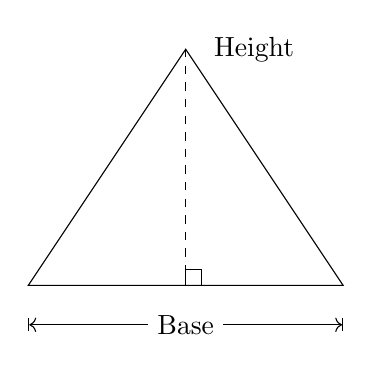
\begin{tikzpicture}

% Define the coordinates for the vertices of the triangle
\coordinate (A) at (0,0);
\coordinate (B) at (4,0);
\coordinate (C) at (2,3);

% Draw the triangle outline
\draw (A) -- (B) -- (C) -- cycle;

% Draw the dashed height line
\draw[dashed] (C) -- ($(A)!(C)!(B)$);

% Draw the right angle symbol at the base of the height
\draw ($(A)!(C)!(B)$) rectangle ++(0.2,0.2);

% Draw the base dimension line with "Base" label
\draw[|<->|] ([yshift=-0.5cm]A) -- ([yshift=-0.5cm]B) node[midway, fill=white] {Base};

% Place the "Height" label at specific coordinates
\node at (3.5,3) [anchor=east] {Height}; % Adjust these coordinates as needed

\end{tikzpicture}
\end{document}